\documentclass{standalone}

\usepackage{tkz-euclide}
\newcommand{\?}{\stackrel{?}{=}}
\newcommand{\vect}[1]{\overrightarrow{#1}}

\begin{document}

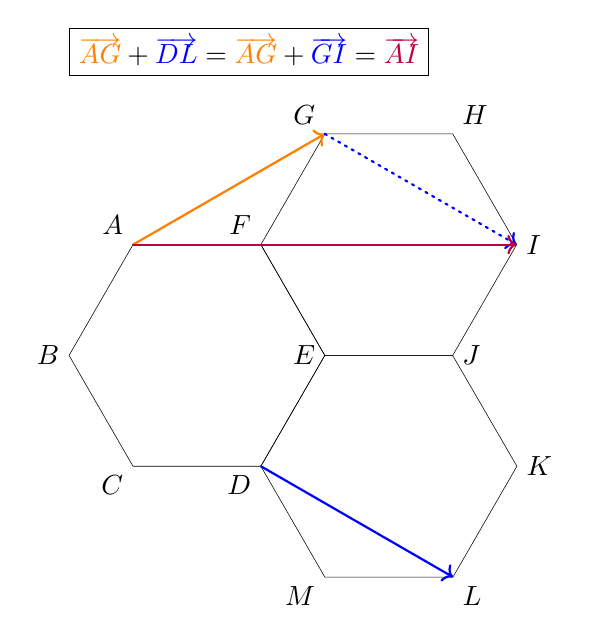
\begin{tikzpicture}[scale=0.35]

% =========================
% POINTS
% =========================

\tkzDefPoint(9,3){A}
\tkzDefPoint(6.68,-1.02){B}
\tkzDefPoint(9,-5.04){C}
\tkzDefPoint(13.64,-5.04){D}
\tkzDefPoint(15.96,-1.02){E}
\tkzDefPoint(13.64,3){F}

\tkzDefPoint(20.6,-1.02){J}
\tkzDefPoint(22.92,3){I}
\tkzDefPoint(20.6,7.02){H}
\tkzDefPoint(15.96,7.02){G}

\tkzDefPoint(15.96,-9.06){M}
\tkzDefPoint(20.61,-9.06){L}
\tkzDefPoint(22.93,-5.04){K}

% =========================
% HEXAGONES
% =========================

\tkzDrawPolygon(A,B,C,D,E,F)
\tkzDrawPolygon(F,E,J,I,H,G)
\tkzDrawPolygon(E,D,M,L,K,J)

% =========================
% LABELS
% =========================

\tkzLabelPoints[above left](A,F,G)
\tkzLabelPoints[above right](H)
\tkzLabelPoints[below left](C,D,M)

\tkzLabelPoints[below right](L)
\tkzLabelPoints[left](B,E)
\tkzLabelPoints[right](J,I,K)

% =========================
% VECTEURS (OPTION A)
% FD - FE = ED
% =========================

% F -> D
\tkzDrawSegment[->,orange,thick](A,G)

% F -> E
\tkzDrawSegment[->,blue,thick](D,L)
\tkzDrawSegment[->,blue,thick, dotted](G,I)

% E -> D
\tkzDrawSegment[->,purple,thick](A,I)

%\tkzDrawSegment[->,green,thick](C,K)

\tkzText[right,draw](6.68,10){${\color{orange}\vect{AG}} + {\color{blue}\vect{DL}} = {\color{orange}\vect{AG}} + {\color{blue}\vect{GI}}={\color{purple}\vect{AI}}$}
\end{tikzpicture}

\end{document}

\vspace{0.5cm}



\end{document}